\chapter{A prototype of a machine learning workflow to classify land use from the housing market dynamics} \label{ch:ml_workflow}

As was previously mentioned in section~\ref{sec:teranet_and_its_challgenges}, one of the major features missing from the available version of Teranet's dataset is the information about the type of property being transacted, which introduces a major limitation on how Teranet's data can be used.
As was described in chapter~\ref{ch:data_preparation}, parcel-level land use information from DMTI and the Department of Geography has been spatially joined to Teranet records, but these sources of land use information also have their limitations:

\begin{itemize}
    \item DMTI's land use data does not offer any split between subcategories of residential properties and only covers the period of 2001--2014
    \item land use from the Department of Geography is a lot more detailed and accurate, but has been collected at a single point in time over the summer of 2012 and 2013
    \item neither of the available land use sources covers the full span of the Longitudinal Housing Market Research conducted by UTTRI (1986-2016)
\end{itemize}

To address this issue, detailed land use from the Department of Geography can be used as labelled data to train a machine learning model capable of recognizing certain property types that have characteristically different behavior on the housing market;
i.e., be able to differentiate a detached house from a condo through such features as high / low volume of transactions, ratio of price to median price for that year, etc.
Chapter~\ref{ch:data_preparation} described the production of the dataset that combines the new engineered Teranet features with spatially-joined variables from Census and TTS\@.
In this chapter, this dataset is used to investigate the opportunity to implement a classification algorithm to determine the parcel land use at Teranet transaction level (recognizing changes of land use with time) based on the housing market dynamics.
This way a machine learning algorithm could be implemented to automate a labour-intensive task of collecting parcel-level detailed land use and expand the accuracy of this data by classifying Teranet records covering the full period of the longitudinal study introduced in section~\ref{subsec:longitudinal_housing_market_research}.

Figure~\ref{fig:typical_ml_workflow} presents a typical workflow for using machine learning in predictive modeling, as summarized by Raschka and Mirjalili\cite{RaschkaMirjalili2017}.

\begin{figure}[hbt!]
    \centering
    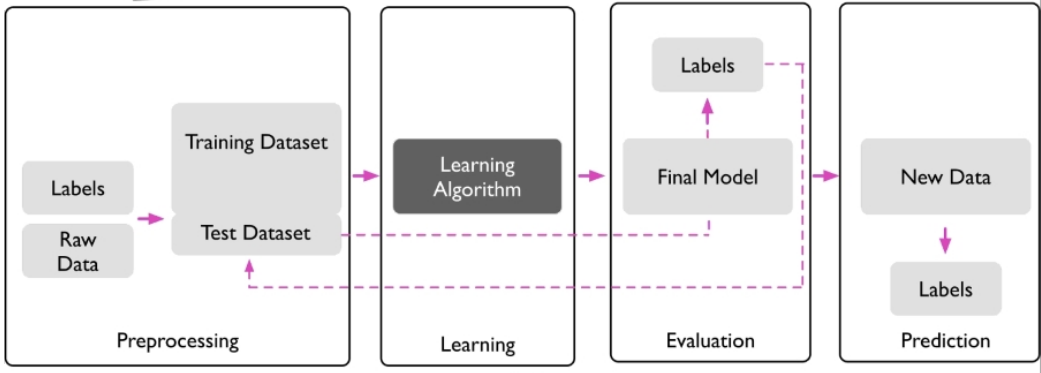
\includegraphics[width=0.98\linewidth,trim=0 0 0 0,clip]{typical_ml_workflow.png}
    \caption{A typical workflow for using machine learning in predictive modeling, as summarized by Raschka and Mirjalili\cite{RaschkaMirjalili2017}.}
    \label{fig:typical_ml_workflow}
\end{figure}

\section{Selecting and encoding target} \label{sec:select_encode_target}

\textit{Classification is a subcategory of supervised learning where the goal is to predict the categorical class labels of new instances, based on past observations. Those class labels are discrete, unordered values that can be understood as the group memberships of the instances. The previously mentioned example of email spam detection represents a typical example of a binary classification task, where the machine learning algorithm learns a set of rules in order to distinguish between two possible classes: spam and non-spam emails.}
The Iris dataset consisting of 150 samples and four features can then be written as a  matrix :


\section{Feature selection} \label{sec:feature_selection}

In the case of 9 features selected via the SBS algorithm, the training subset of Teranet dataset consists of 138,015 samples and 9 features that can be written as a $138015 \times 9$ matrix $\boldsymbol{X} \in \mathbb{R}^{138015 \times 9}$:

\vspace{5mm}
\begin{bmatrix}
    \centering
    x_1^{(1)} & x_2^{(1)} & \dots & x_9^{(1)} \\ \\
    x_1^{(2)} & x_2^{(2)} & \dots & x_9^{(2)} \\ \\
    \vdots & \vdots & \vdots & \vdots \\ \\
    x_1^{(138015)} & x_2^{(138015)} & \dots & x_9^{(138015)}
\end{bmatrix},$
\vspace{1mm}

where superscript refers to the training sample, and the subscript refers to the dimension of the training dataset.


\section{Training, testing and validating the model} \label{sec:train_test_validate_model}

\section{Feature scaling} \label{sec:feature_scaling}

\section{Classification algorithms and their performance} \label{sec:classification_algorithms_performance}

No Free Lunch Theorem by David H. Wolpert states that no single classifier works best across all possible scenarios\cite{Wolpert1996}, as there is a lack of a priori distinctions between learning algorithms.

\section{Chapter summary} \label{ml_workflow_summary}